%\documentclass[a4,semhelv,landscape]{seminar}
\documentclass[landscape]{slides}
%\documentclass[pdf, default, slideBW, nocolorBG]{prosper}
\usepackage[left=1.0cm,top=0.2cm,right=1.0cm,nohead,nofoot]{geometry}
%\def\everyslide{\sffamily}
%\usepackage{fullpage}
\usepackage{graphicx}
\usepackage{setspace}
\usepackage{color}
\usepackage{fancyvrb}
\usepackage{verbatim}
\usepackage{nopageno}
%\usepackage{times}
% define some nice colors
\definecolor{myred}{rgb}{0.6,0,0}
\definecolor{myblue}{rgb}{0,0.2,0.4}
\def\imagetop#1{\vtop{\null\hbox{#1}}}
%\color{myblue}

%\DefineVerbatimEnvironment{sreoutput}{Verbatim}{fontsize=\scriptsize,xleftmargin=10.0\parindent}%
\DefineVerbatimEnvironment{sreoutput}{Verbatim}{fontsize=\small,xleftmargin=10.0\parindent}%
\DefineVerbatimEnvironment{sreoutput2}{Verbatim}{fontsize=\tiny,xleftmargin=10.0\parindent}%
%\input{macros}

\begin{document}
%%%%%%%%%%%%%%%%%%%%%%%%%%%%%%%%%%%%%%%%%%%%%%%%%%%%%%%%%%%%%%%%%%%%
%Slide 0 - title
\begin{slide}
\begin{center}
\large{\textbf{Covariance models and Infernal 1.1}}

\normalsize

Eric Nawrocki

Sean Eddy's Lab

%10.05.11

\medskip

\medskip

\small

\begin{tabular}{c}
Howard Hughes Medical Institute \\ 
Janelia Farm Research Campus \\
\\
%Deparment of Genetics \\
%Washington University in St. Louis \\
%\\
\end{tabular}

\vspace{0.1in}

%\includegraphics[width=2.5in]{figs/janelia-logo}
%\hspace{2in}
%\includegraphics[width=1.75in]{figs/washu}
\end{center}
\end{slide}
%%%%%%%%%%%%%%%%%%%%%%%%%%%%%%%%%%%%%%%%%%%%%%%%%%%%%%%%%%%%%%%%%%%%
\begin{slide}
\begin{center}
%\textbf{Comparative analysis of sequence families}: \\
\textbf{Sequence conservation provides \\ information for homology searches}
%\emph{Functionally important sequence features are evolutionarily conserved.}
\medskip

%A simple, made-up RNA family:

%Evolution conserves functionally \\ important sequence features.

%Evolution conserves sequence \\ based on its functional importance.

Conservation levels vary across alignment columns.

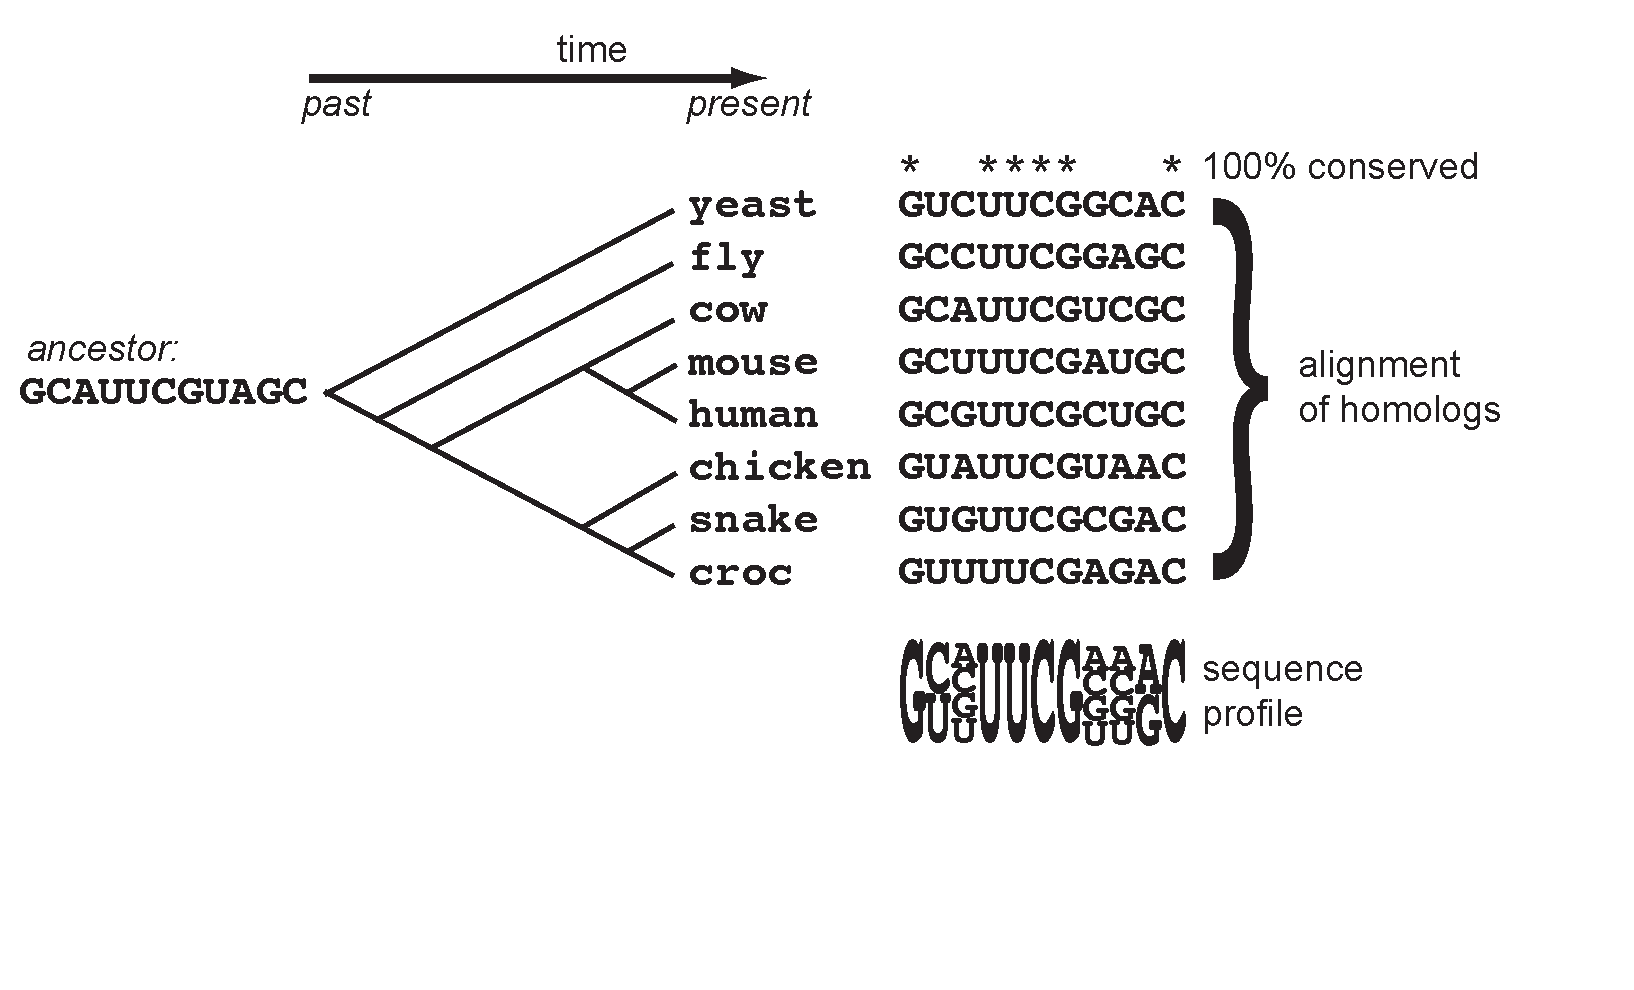
\includegraphics[width=9in]{figs/seqstructprofiles-seq1}
%\includegraphics[width=9in]{figs/tmp}
\end{center}

\vfill
\end{slide}
%%%%%%%%%%%%%%%%%%%%%%%%%%%%%%%%%%%%%%%%%%%%%%%%%%%%%%%%%%%%%%%%%%%%%%
\begin{comment}
\begin{slide}
\begin{center}
\textbf{Structure conservation provides additional information}
\medskip

Base-paired positions covary \\ to maintain Watson-Crick complementarity.

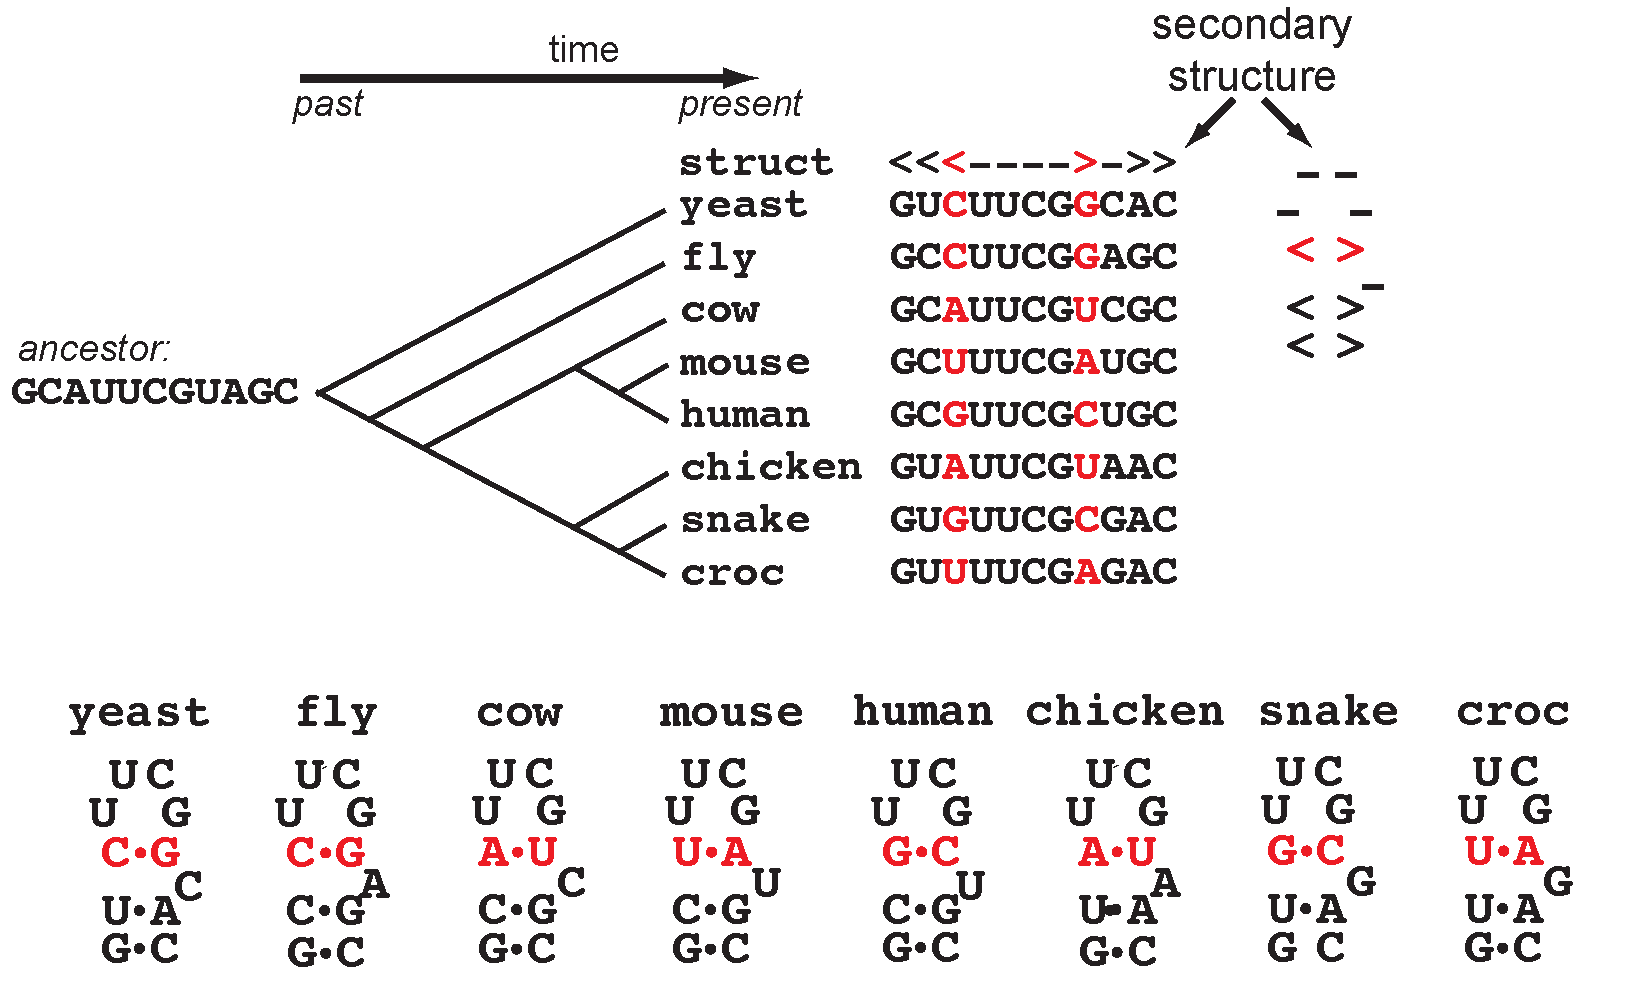
\includegraphics[width=9in]{figs/seqstructprofiles-struct1}
\end{center}

\vfill
\end{slide}
\end{comment}
%%%%%%%%%%%%%%%%%%%%%%%%%%%%%%%%%%%%%%%%%%%%%%%%%%%%%%%%%%%%%%%%%%%%%%
\begin{slide}
\begin{center}
\textbf{Structure conservation provides additional information}
\medskip

Base-paired positions covary \\ to maintain Watson-Crick complementarity.

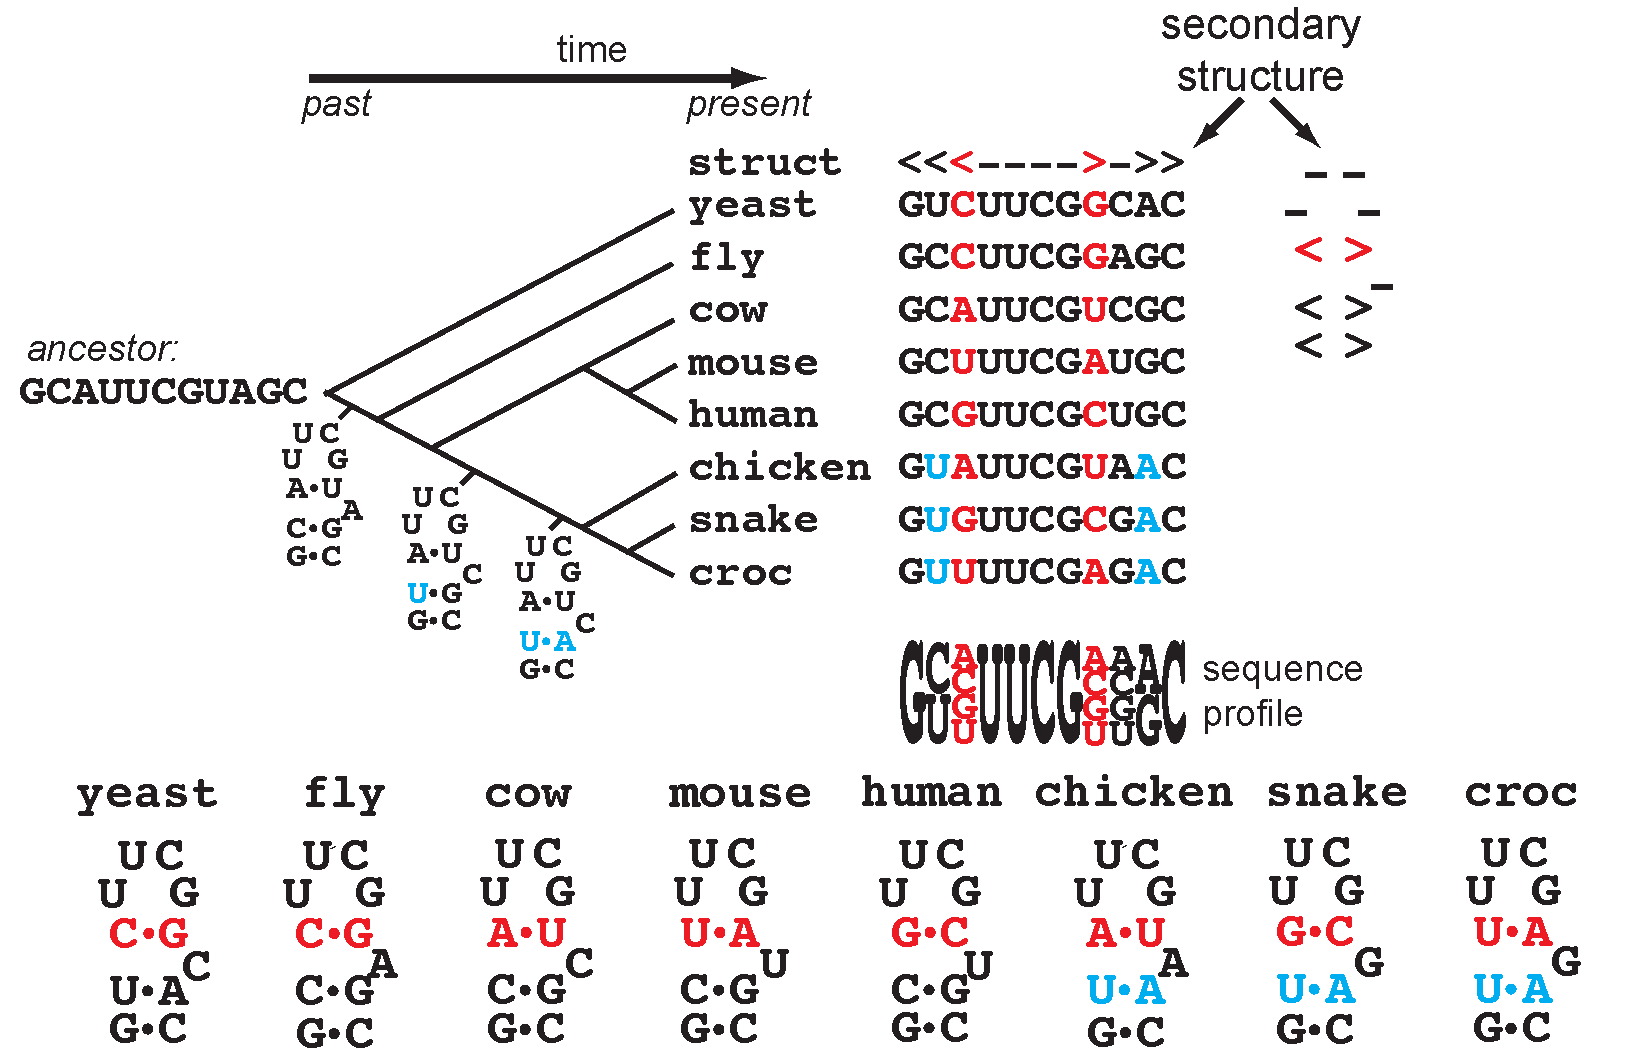
\includegraphics[width=9in]{figs/seqstructprofiles-struct2}
\end{center}

\vfill
\end{slide}
%%%%%%%%%%%%%%%%%%%%%%%%%%%%%%%%%%%%%%%%%%%%%%%%%%%%%%%%%%%%%%%%%%%%%%%%%%
\begin{slide}
\begin{center}
\textbf{Levels of sequence and structure conservation in RNA families}
\end{center}
\medskip

\begin{center}
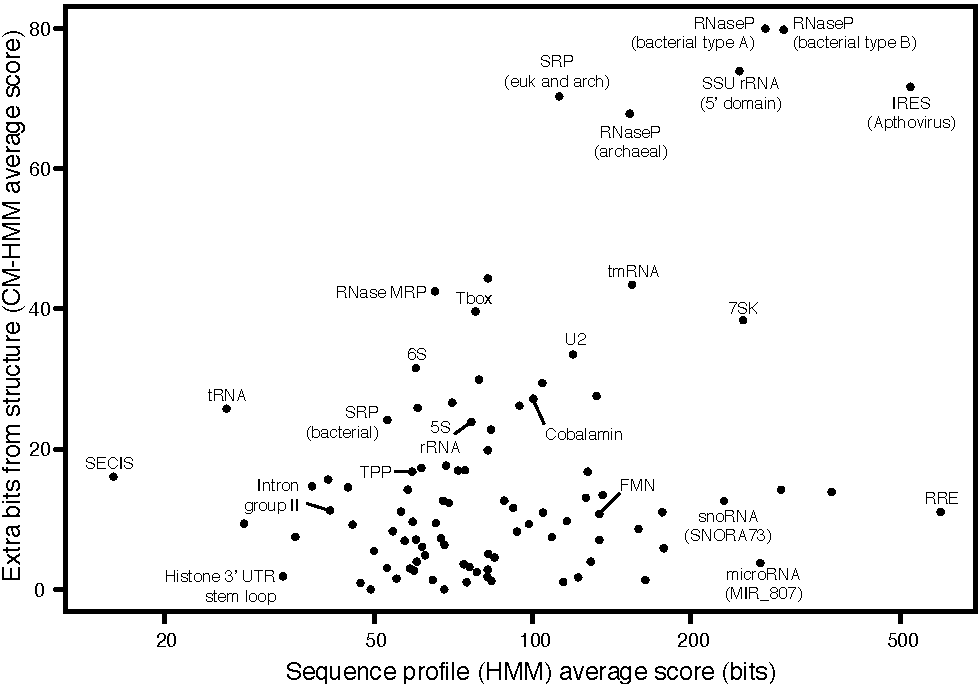
\includegraphics[height=6.5in]{figs/avgscores}
\end{center}

\vfill

\end{slide}
%%%%%%%%%%%%%%%%%%%%%%%%%%%%%%%%%%%%%%%%%%%%%%%%%%%%%%%%%%%%%%%%%%%
\begin{slide}
\begin{center}
%\textbf{profile HMMs and covariance models}
\textbf{Eddy lab software for profile probabilistic models} \\
(since 1994)
\end{center}
\medskip

\begin{center}
\small
\begin{tabular}{r|cc} 
%             &         & sequence \\
%             & sequence& and structure \\
%             & profiles& profiles \\ \hline
             & sequence & sequence and \\
             & profiles & structure profiles \\ \hline
  \\
  models     & profile HMMs     & {\color{red} covariance models (CMs)} \\ 
  \\
  software   & {\sc HMMER}      & {\sc Infernal} \\ 
             &                  & (prev. COVE) \\
  \\
  main use   & proteins         & RNAs \\ 
  \\
  database   & {\sc Pfam}       & {\sc Rfam} \\
             & (12273 families) & (1973 families) \\
  \\
%  primary sequence & yes & yes \\
%  \\
%  secondary structure & no & yes \\
%  \\
%  algorithms & Viterbi, Forward & CYK, Inside \\
%%             & Forward & Inside \\
%             &         & \\
%  complexity & $O(LN)$ & $O(LN^{2} log N)$ \\
%  \\
  performance& faster but    & slower but    \\
  for RNAs   & less accurate & more accurate \\
\end{tabular}

%\hspace{1.2in}
\includegraphics[height=2in]{figs/hmmer_logo}\hspace{1.05in}\includegraphics[height=2.6in]{figs/infernal_logo}
\hspace{1.2in}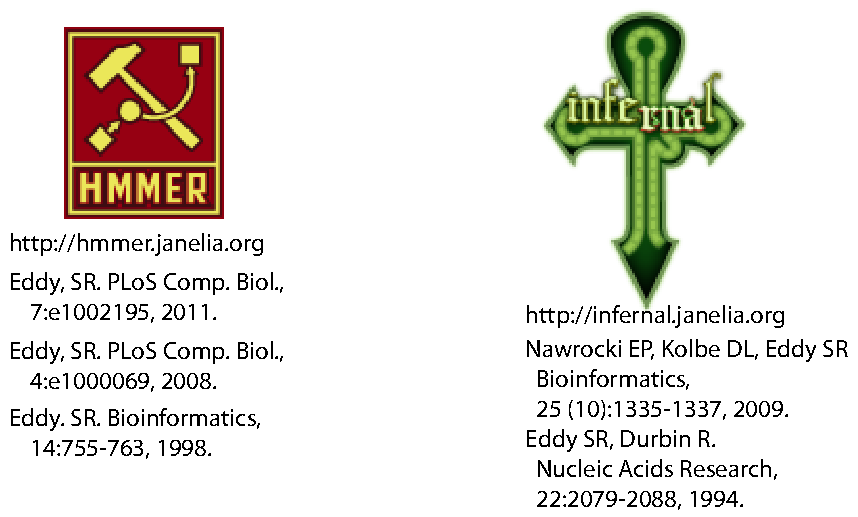
\includegraphics[height=2.7in]{figs/hmmer-infernal-refs}

\end{center}

\vfill

\end{slide}
%%%%%%%%%%%%%%%%%%%%%%%%%%%%%%%%%%%%%%%%%%%%%%%%%%%%%%%%%%%%%%%
%%%%%%%%%%%%%%%%%%%%%%%%%%%%%%%%%%%%%%%%%%%%%%%%%%%%%%%%%%%%%%%%%%%%
\begin{slide}
\begin{center}
%\textbf{profile HMMs and covariance models}
\textbf{Profile HMMs: sequence family models built from alignments}
\end{center}
\medskip

\center{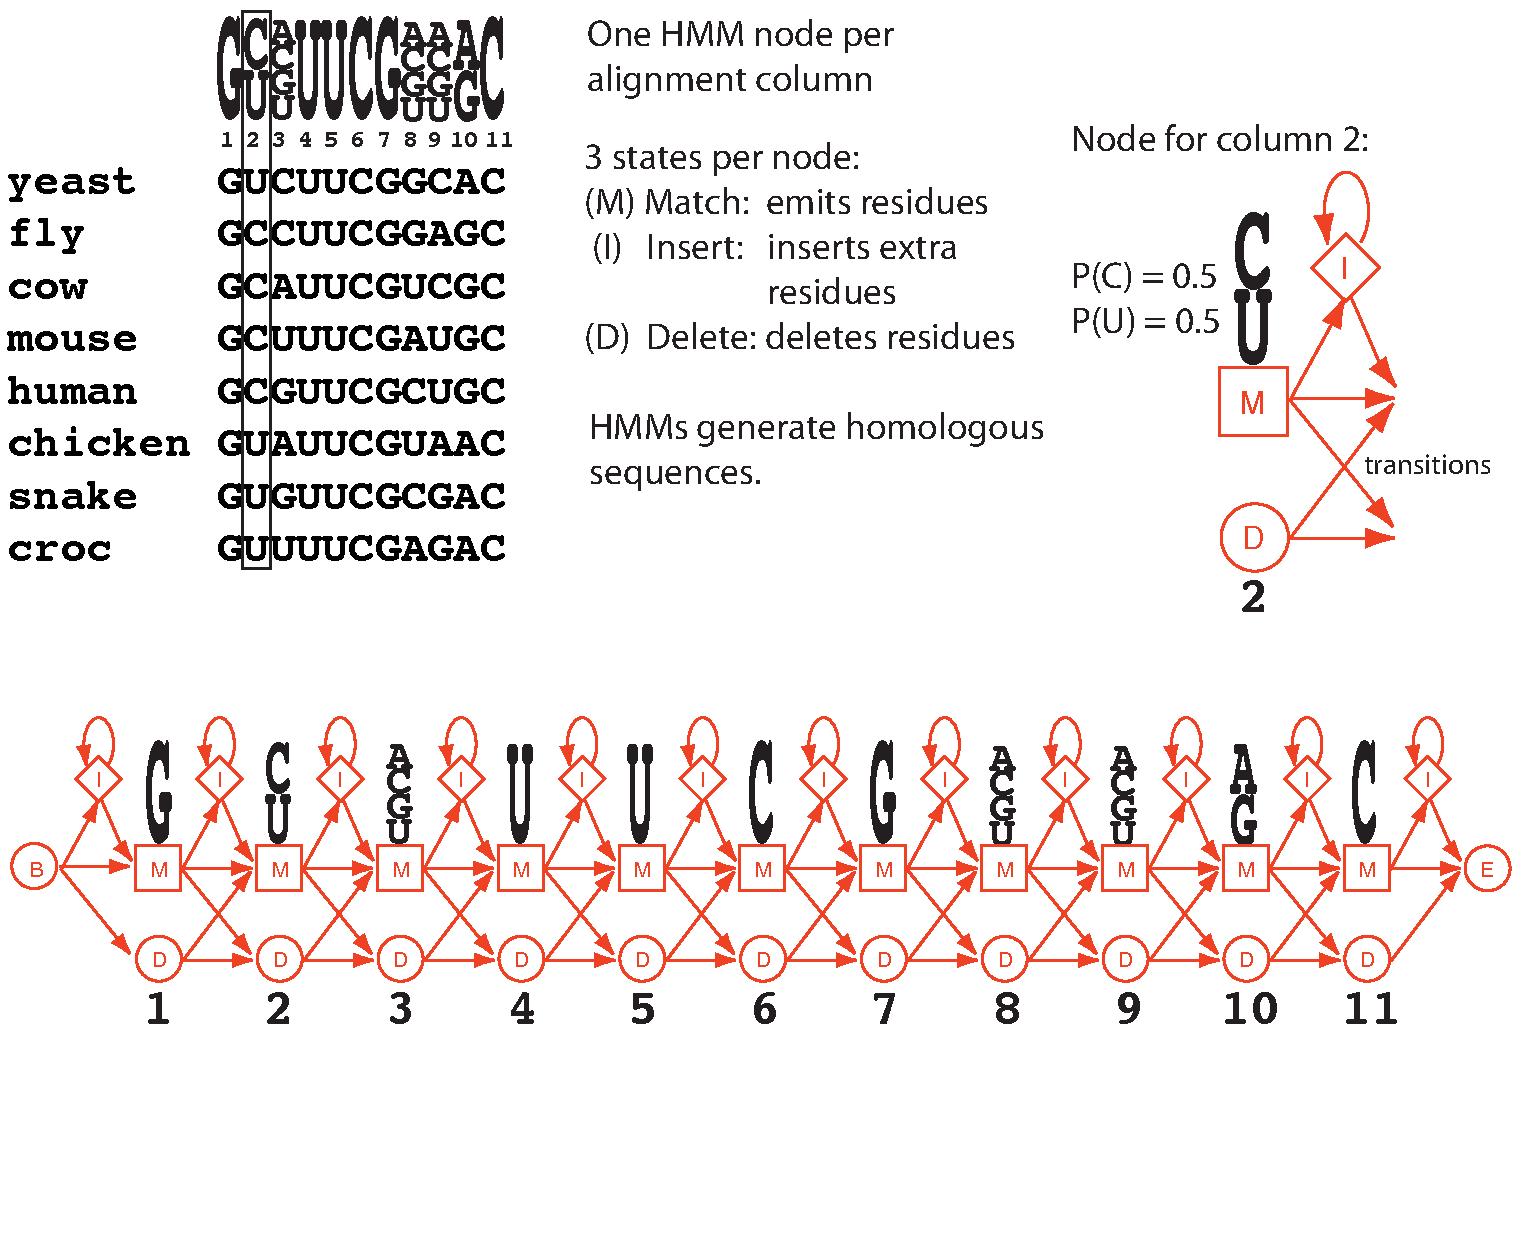
\includegraphics[height=7in]{figs/hmm}}

%An HMM generates ``homologous'' sequences.

\end{slide}
%%%%%%%%%%%%%%%%%%%%%%%%%%%%%%%%%%%%%%%%%%%%%%%%%%%%%%%%%%%%%%%
\begin{slide}
\begin{center}
%\textbf{profile HMMs and covariance models}
\textbf{Profile HMMs: sequence family models built from alignments}
\end{center}
\medskip

\center{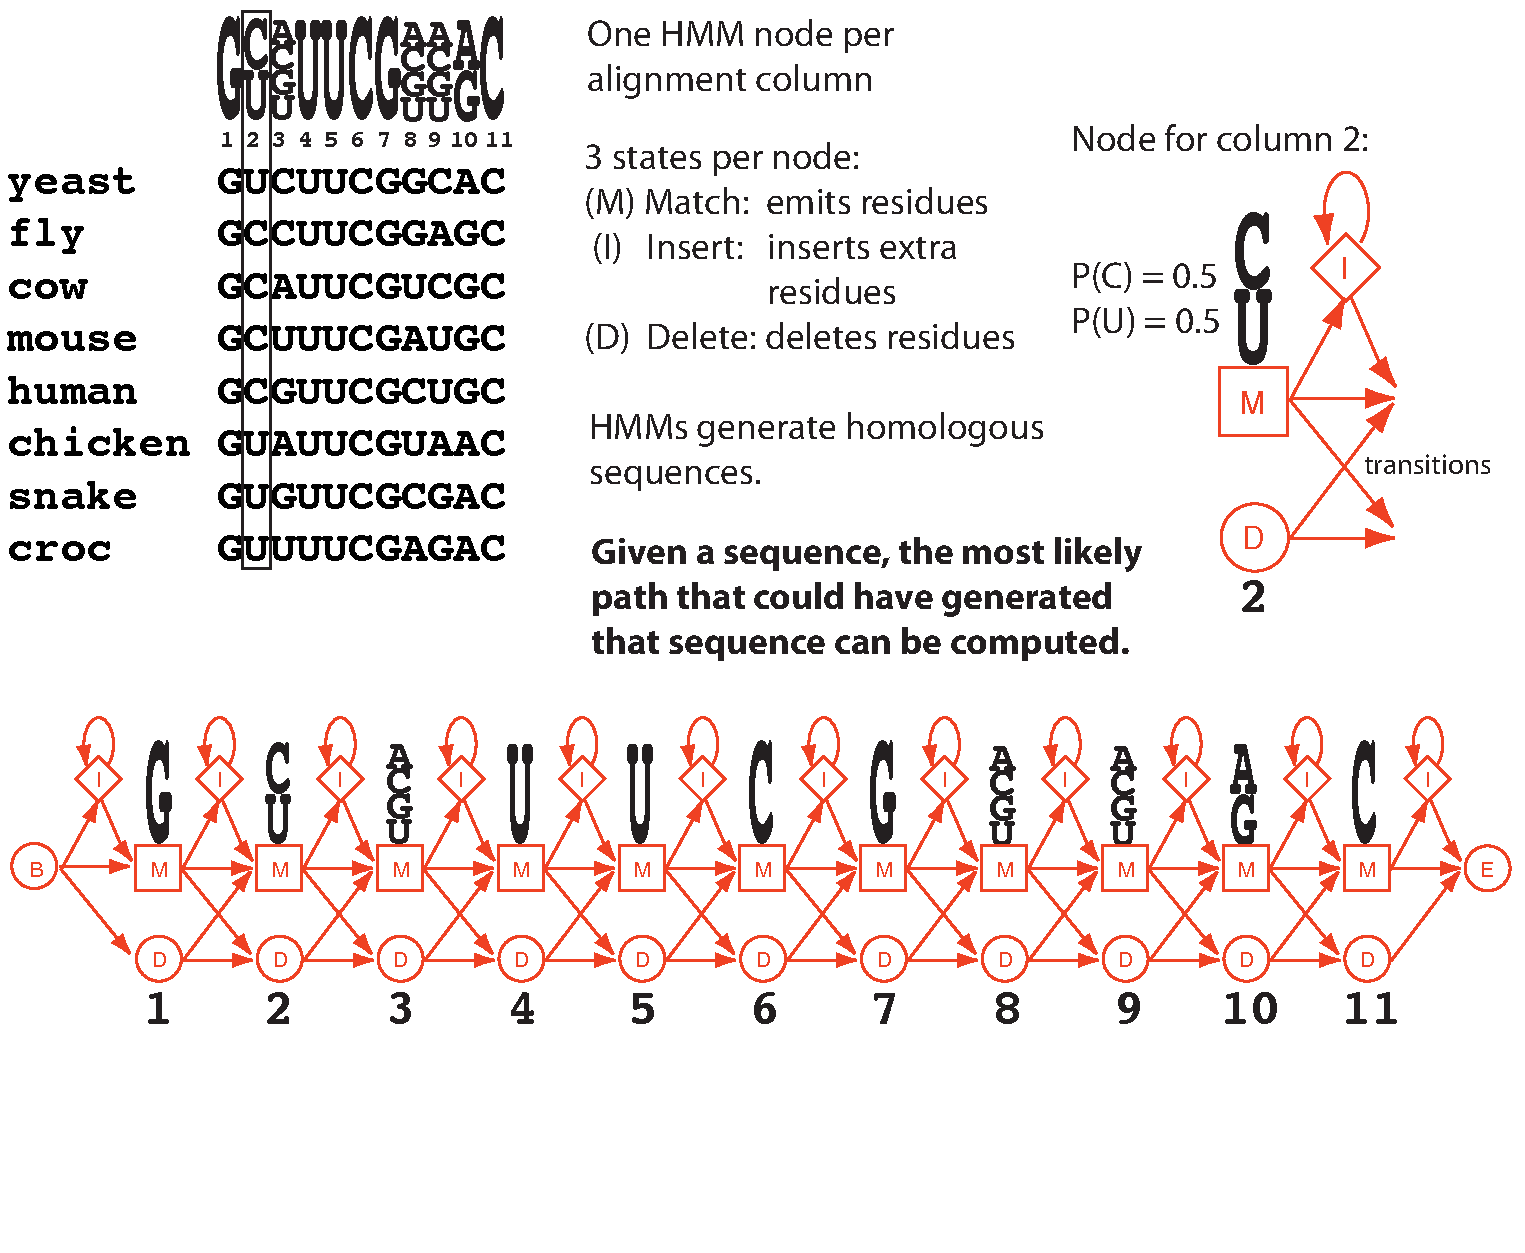
\includegraphics[height=7in]{figs/hmm-given}}
\end{slide}
%%%%%%%%%%%%%%%%%%%%%%%%%%%%%%%%%%%%%%%%%%%%%%%%%%%%%%%%%%%%%%%
\begin{slide}
\begin{center}
%\textbf{profile HMMs and covariance models}
\textbf{Profile HMMs: sequence family models built from alignments}
\end{center}
\medskip

\center{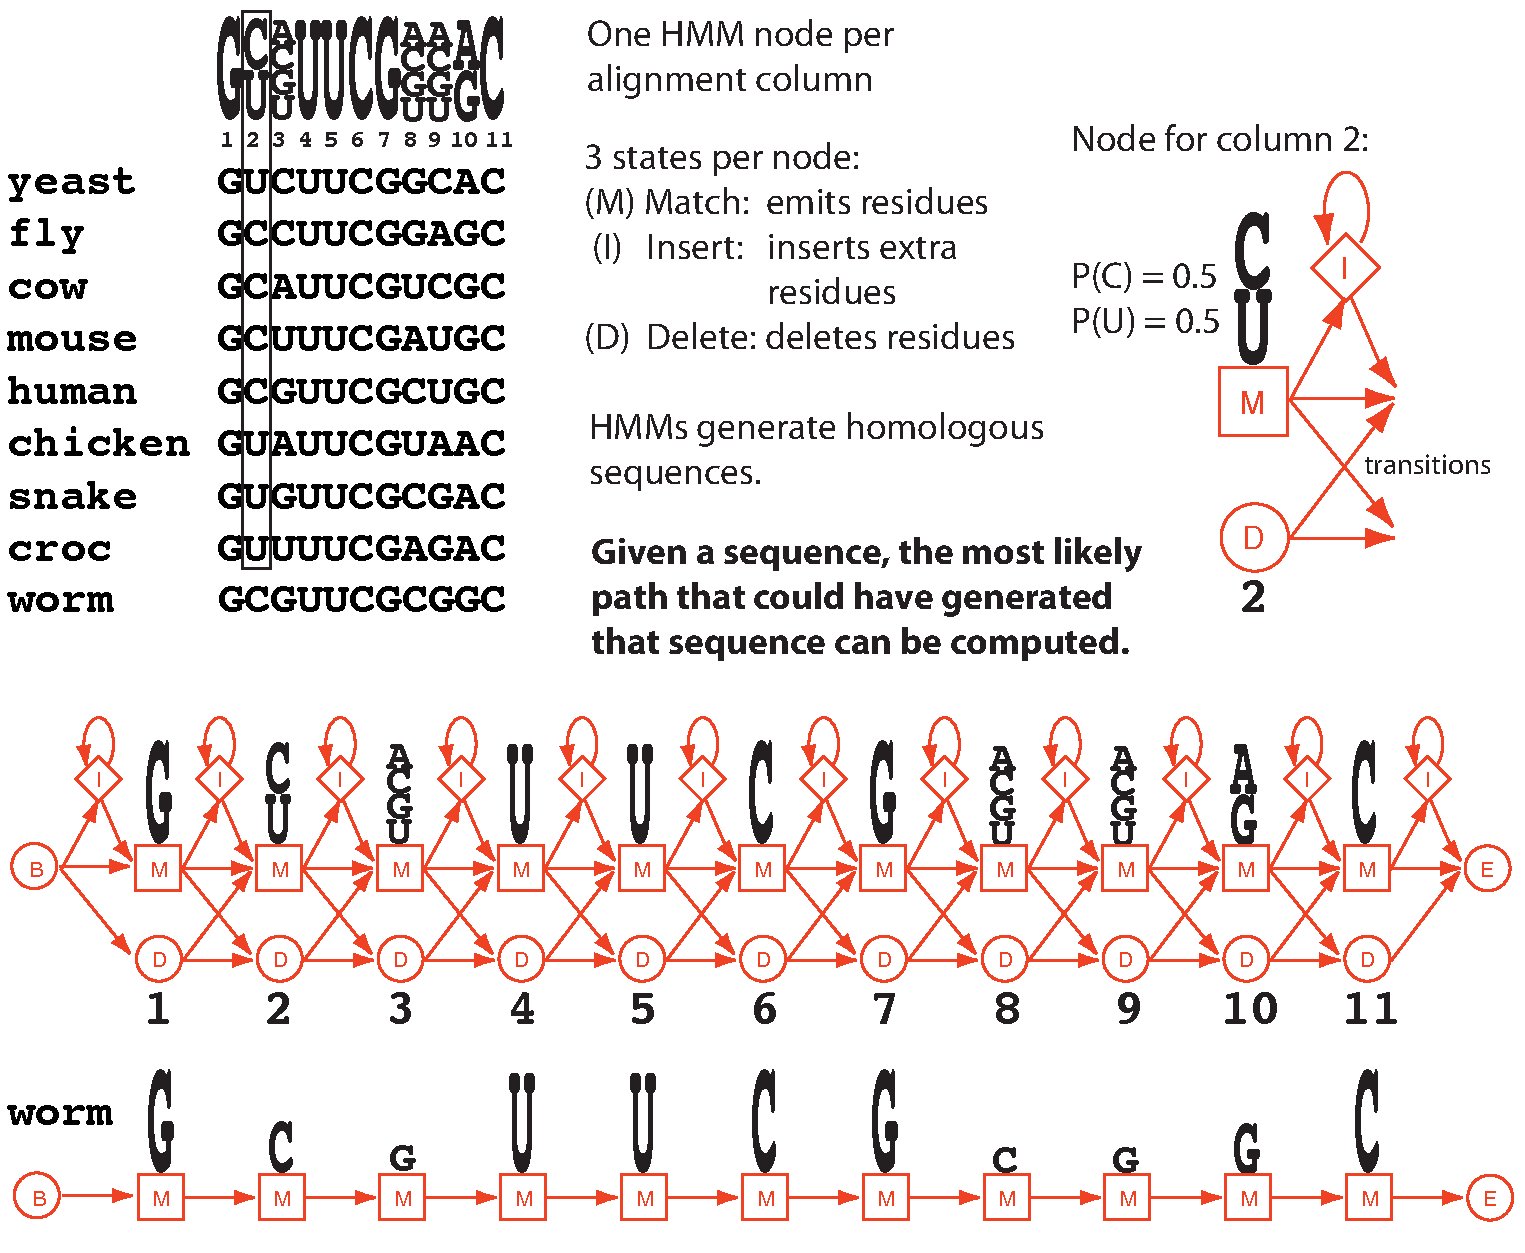
\includegraphics[height=7in]{figs/hmm-worm}}
\end{slide}
%%%%%%%%%%%%%%%%%%%%%%%%%%%%%%%%%%%%%%%%%%%%%%%%%%%%%%%%%%%
\begin{slide}
\begin{center}
%\textbf{profile HMMs and covariance models}
\textbf{Profile HMMs: sequence family models built from alignments}
\end{center}
\medskip

\center{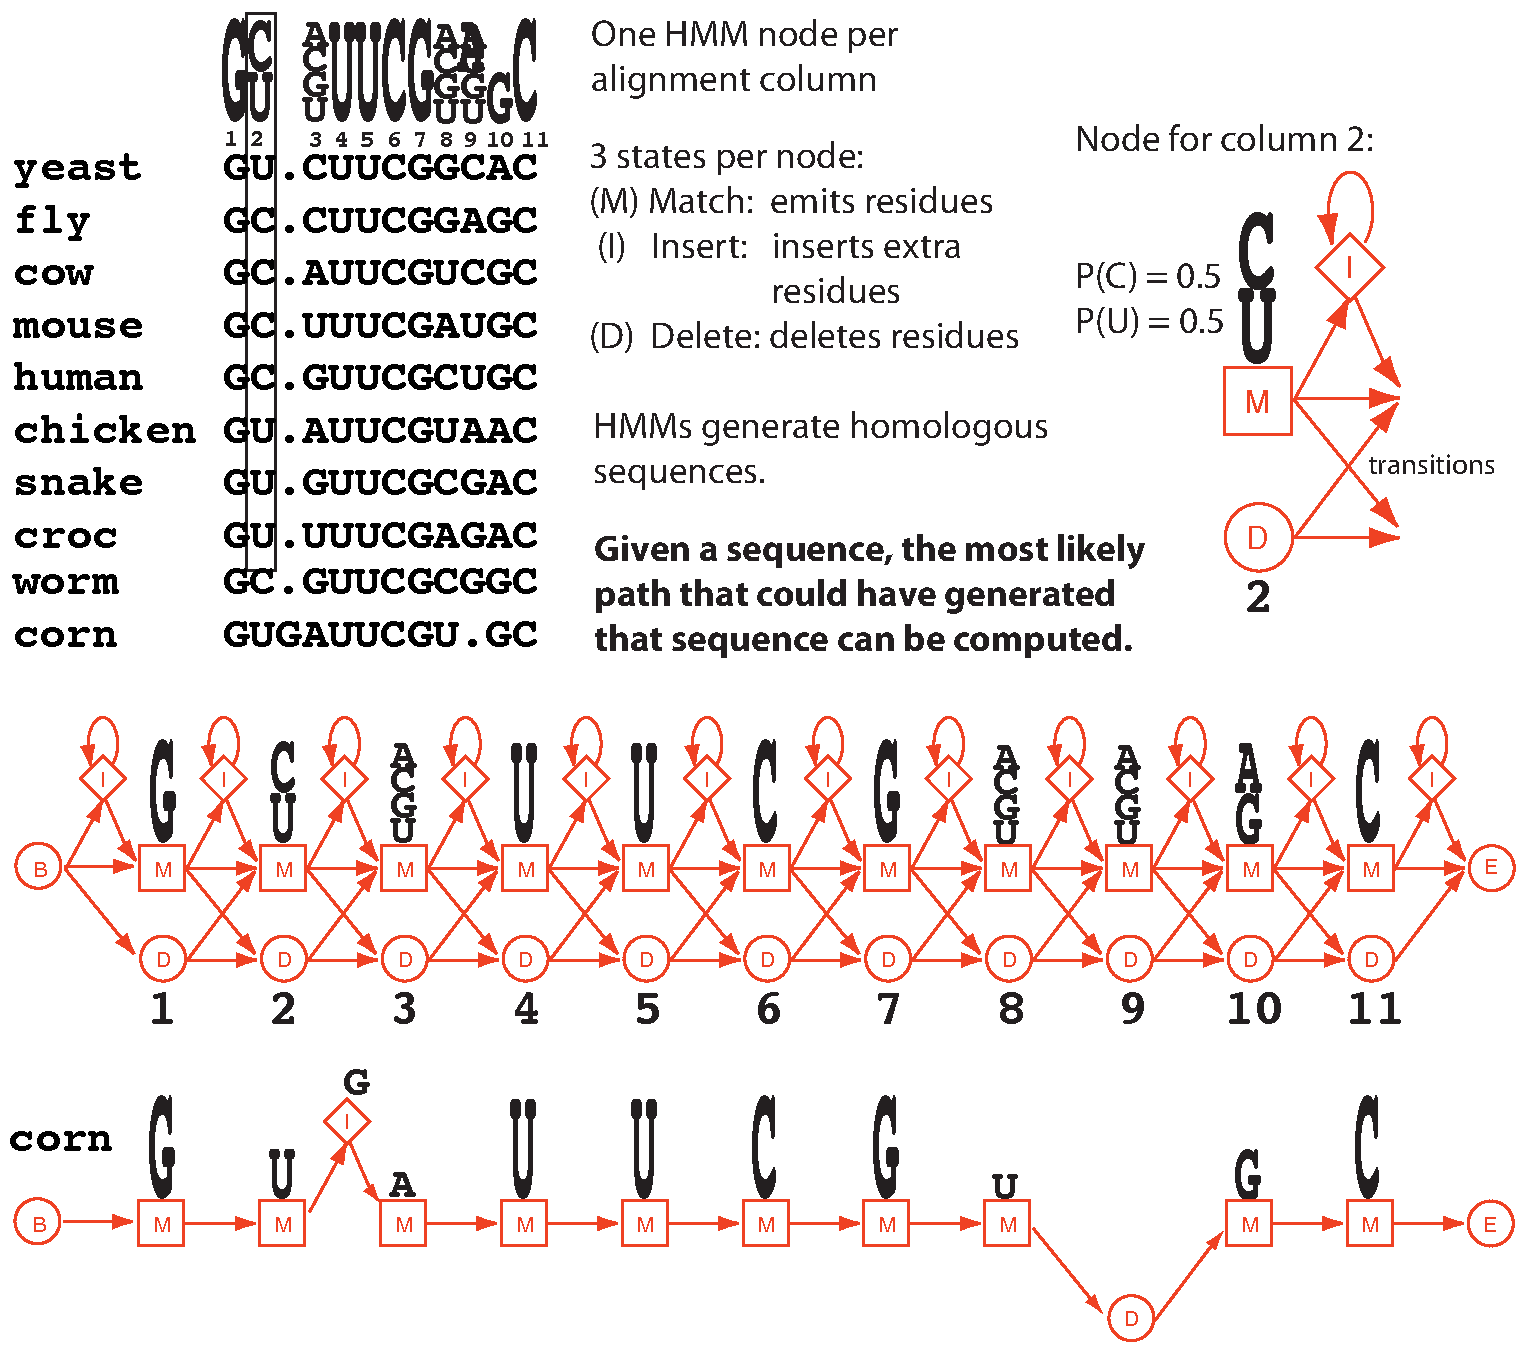
\includegraphics[height=7in]{figs/hmm-corn}}
\end{slide}
%%%%%%%%%%%%%%%%%%%%%%%%%%%%%%%%%%%%%%%%%%%%%%%%%%%%%%%%%%%%%%%
\begin{slide}
\begin{center}
%\textbf{profile HMMs and covariance models}
\textbf{Covariance models (CMs) are built \\ from structure-annotated alignments}
\end{center}
\medskip

\center{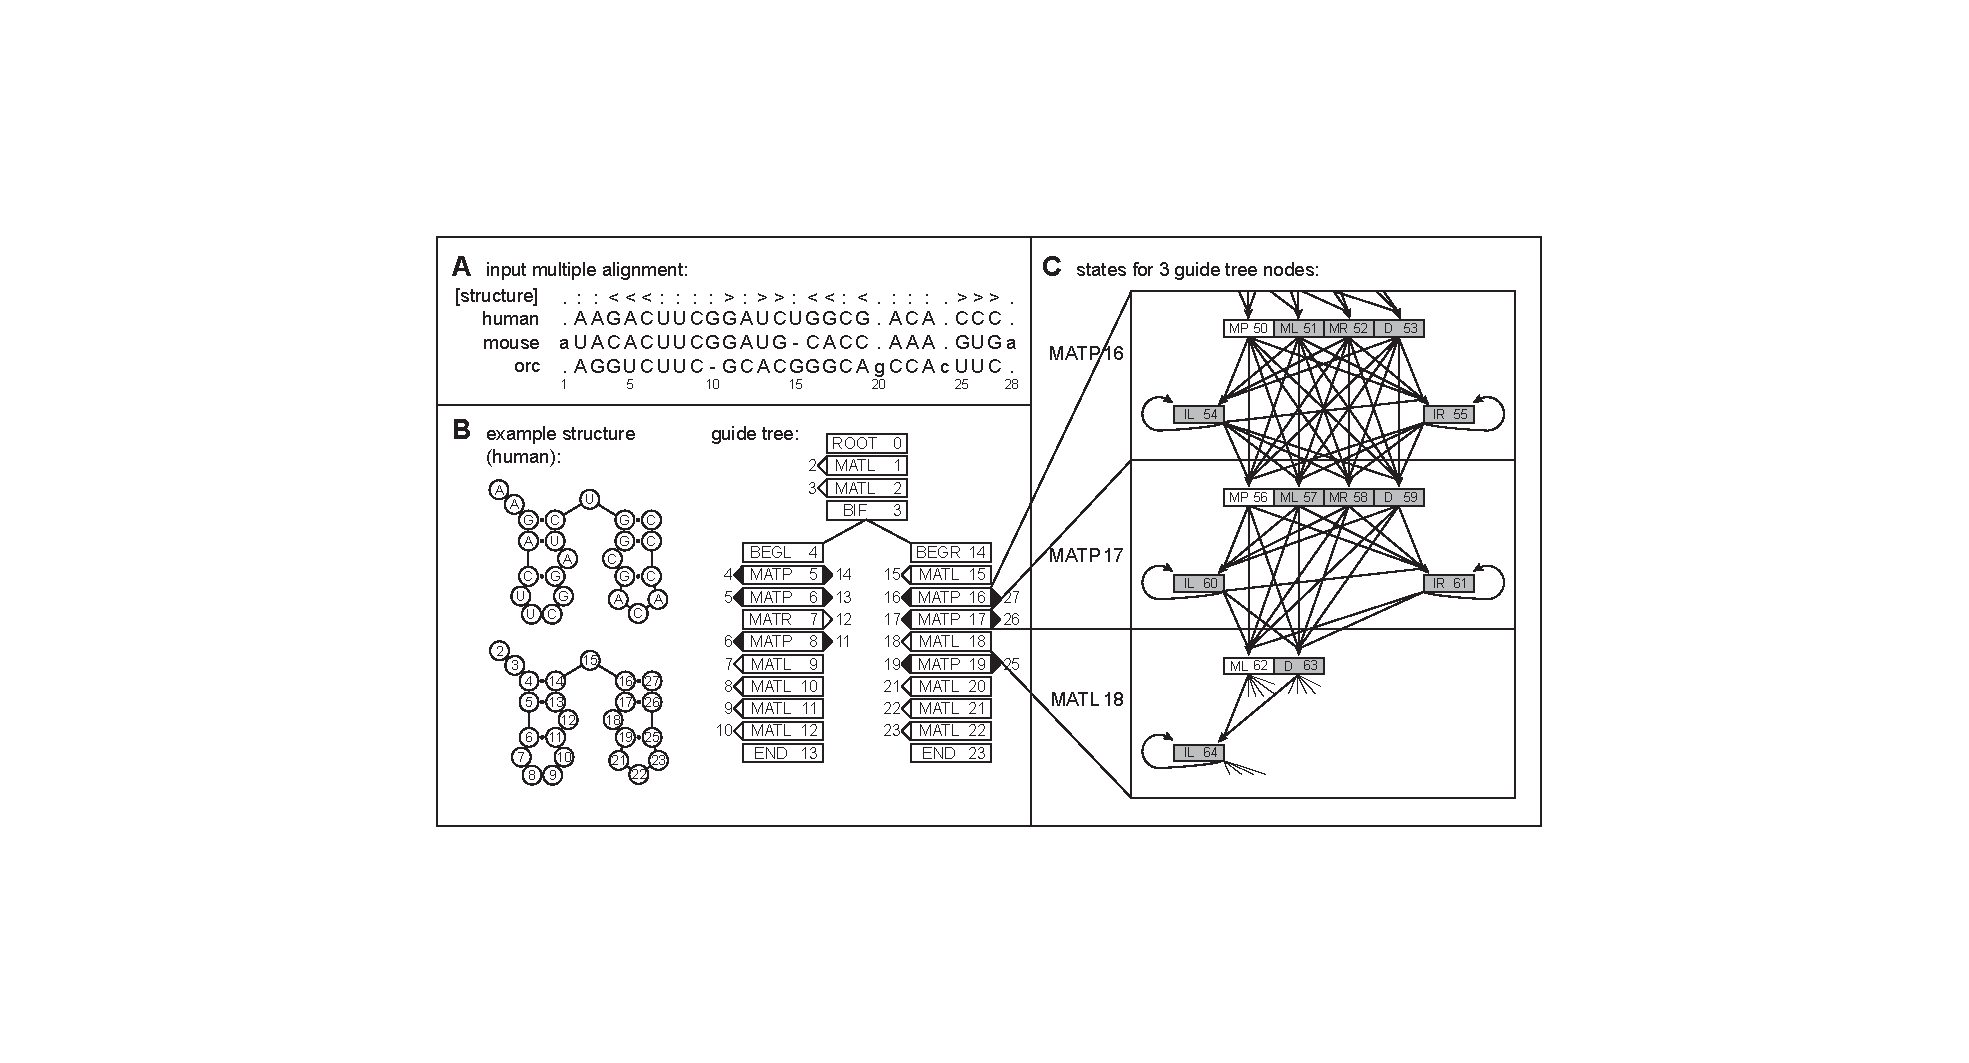
\includegraphics[width=8in]{figs/cmintro_bandcyk}}

\center{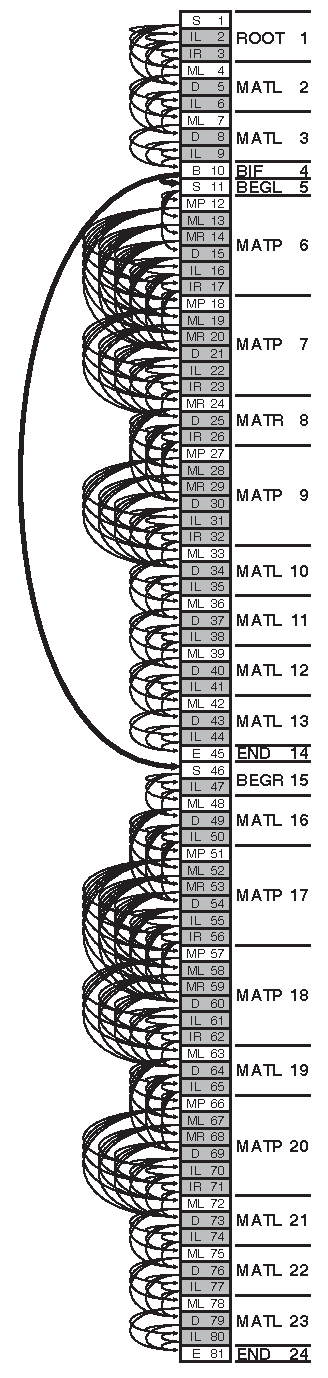
\includegraphics[width=2in,angle=270]{figs/cm-graph-small}}

%\item Extensions of profile HMMs that 

%\item Generative models that generate ``homologous'' structural RNA sequences

\vfill

\end{slide}
%%%%%%%%%%%%%%%%%%%%%%%%%%%%%%%%%%%%%%%%%%%%%%%%%%%%%%
\begin{slide}
\begin{center}
\textbf{CM searches are slow (especially for large RNAs)}
\end{center}

\small
%For a:
%
%\begin{tabular}{l}
%Model of $M$ positions, \\
%a maximum hit length of $W$ nucleotides, \\
%and a database of length $L$: \\
%\end{tabular}

\begin{center}
\begin{tabular}{rcll}
model & DP algorithms & direction & complexity \\ \hline
& & & \\
profile HMM & Viterbi, Forward & left to right     & $O(N^2)$      \\
& & & \\
         CM & CYK, Inside      & inside to outside & $O(N^3logN)$ \\
%& & & \\
%& & & \\
%\multicolumn{4}{l}{$L$: database length} \\
%\multicolumn{4}{l}{$M$: model length} \\
%\multicolumn{4}{l}{$W$: maximum hit length} \\

& & & \\
& & & \\
& & & \\
\multicolumn{4}{l}{CYK and Inside fill in a 3-dimension matrix with
  $(v,i,j)$ tuples:} \\
\end{tabular}

\medskip

\includegraphics[width=8in]{figs/cm-hmm-complexity}

\end{center}
\vfill

\end{slide}
%%%%%%%%%%%%%%%%%%%%%%%%%%%%%%%%%%%%%%%%%%%%%%%%%%%%%%
\begin{slide}
\begin{center}
\textbf{Accelerating CM searches: filtering and banded DP}
\end{center}

%\item
%  Query-dependent banding (QDB) accelerates
%  homology search six-fold at a negligible cost to sensitivity
\small
\begin{itemize}
\item
  Filtering: search database with faster method first, hits above some threshold \\ survive the filter and are searched with the slow CM.
  \begin{itemize}
  \item
    \emph{tRNAscan-SE}\footnote{Lowe T, Eddy S, NAR 25:955-964, 1997}:
    filters database using tRNA-specific heuristics (1997)
  \item
    Rfam uses BLAST filters (2002-present)
  \item
    Weinberg and Ruzzo\footnote{Weinberg Z, Ruzzo WL. Bioinformatics 22(1):35–39,
      2006.} developed HMM filters for faster searches (2004, 2006).
  \item
    Others have also worked on this (Sun and Buhler 
    \footnote{Sun Y, Buhler J, Comput. Systems
      Bioinf., p145-156, 2008.}, Zhang and Bafna\footnote{Zhang S et al.,
      Bioinformatics. 22(14):e557-e565, 2006.})
  \end{itemize}
\item
  Query dependent banding (QDB)\footnote{Nawrocki and Eddy, PLoS Comp
  Bio, 2007}: restrict subsequence lengths that can align to
  each state of the model.
%  \begin{itemize}
%    Empirical time complexity drops from $O(LMWlogW)$ to $O(LMKlogW)$
\item Infernal 1.0: HMM filtering and QDB yield 100-fold acceleration (2009)
\end{itemize}

\vfill

\end{slide}
%%%%%%%%%%%%%%%%%%%%%%%%%%%%%%%%%%%%%%%%%%%%%%%%%%%%%%

%%%%%%%%%%%%%%%%%%%%%%%%%%%%%%%%%%%%%%%%%%%%%%%%%%%%
\begin{slide}
\begin{center}
\textbf{RMARK: an internal RNA homology search benchmark}
\end{center}
\medskip
\begin{minipage}{7in}
\small
\begin{itemize}
%\item
%  BRaliBase III is too easy (Freyhult \& Gardner, Genome Research, 2007)
\item
  RMARK construction - for each of the 503 Rfam 7.0 seed alignments:
  \begin{itemize}
%  \item
%    remove sequences $<$ 70\% average family length
  \item 
    single-linkage cluster sequences by sequence identity \\ given the alignment
  \item 
    look for a \textcolor{blue}{training} cluster and
    \textcolor{red}{testing} cluster such that: 
    \begin{itemize}
    \item
      no \textcolor{blue}{training}/\textcolor{red}{test} sequence pair is $>$ 60\% identical
%    \item
%      at least five sequences are in the \textcolor{blue}{training} set
%    \item
%      every seed sequence is either a training or testing sequence
    \end{itemize}
  \item
    filter \textcolor{red}{test} set so no two test seqs $>$ 70\% identical 
  \item
    51 families qualify, with 450 \textcolor{red}{test} sequences
    %106 families qualify, with 780 test sequences
  \item
    %\textcolor{red}{test} seqs are embedded in a 1 Mb pseudo-genome (25\% A,C,G,U)
    test seqs are embedded in a 10 Mb (20 Mb counting both strands) pseudo-genome of ``realistic''
    base composition (RMARK2)
%  \item
%    %\textcolor{red}{test} seqs are embedded in a 1 Mb pseudo-genome (25\% A,C,G,U)
%    previously (RMARK1) test seqs were embedded in a 1 Mb pseudo-genome of 25\% A,C,G,U
  \end{itemize}
\end{itemize}
\vspace{1.0in}
\end{minipage}
\hspace{0.1in}
\begin{minipage}{3.5in}
  Example: 
\vspace{0.2in}

\begin{center}
\includegraphics[height=7in]{figs/u8-RF00373-tree}

\end{center}
\end{minipage}
\end{slide}
%%%%%%%%%%%%%%%%%%%%%%%%%%%%%%%%%%%%%%%%%%%%%%%%%%%%%%%%%%%%%%%%%%%

\begin{slide}
\center{\includegraphics[width=10.2in]{figs/fp-roc}}
\vfill 
\end{slide}
%%%%%%%%%%%%%%%%%%%%%%%%%%%%%%%%%%%%%%%%%%%%%%%%%%%%%%%%%%%%%%%%%%%%%%%%%%
\begin{slide}
\begin{center}
\textbf{100 to 1000-fold faster profile HMM searches using HMMER3} \\
(Eddy, PLoS Comp Bio, 2011) 
\end{center}
\medskip

\small
\begin{itemize}
\item Striped vector parallelization (Farrar, Bioinformatics, 2007)
\end{itemize}

\center{\includegraphics[height=6in]{figs/eddy11-fig4}}
\vfill 
\end{slide}
%%%%%%%%%%%%%%%%%%%%%%%%%%%%%%%%%%%%%%%%%%%%%%%%%%%%%%%%%%%%%%%%%%%%%%%%%%
\begin{slide}
\begin{center}
\textbf{Infernal 1.1's HMMER3-based cmsearch pipeline}
\medskip

%\scriptsize
\tiny
\begin{tabular}{ll||r|r|r}
  & model         & hmmer3 & infernal 1.1 \\ \hline
& & & \\
F1 (MSV/SSV)  & HMM & P=0.02     & P=0.35 \\
& & & \\
\multicolumn{2}{c||}{\emph{windows $>$ 2*W are split up}} & & & \\
& & & \\
F2 (Viterbi) & HMM & P=0.001    & P=0.15 \\
& & & \\
F3 (Forward) & HMM & P=0.00001  & P=0.003 \\
& & & \\
F4 (glocal Forward) & HMM &     & P=0.003 \\
& & & \\
\multicolumn{2}{c||}{\emph{overlapping windows are merged}} & & & \\
& & & \\
F5 (glocal envelope defn)  & HMM & & P=0.003 \\
& & & \\
F6 (HMM banded CYK)  & CM &    & P=0.0001 \\
& & & \\
F7 (HMM banded Inside)& CM &  &      \\ %\hline
%& & & \\
%& & & \\
%Avg model per Gb time   & & 0.02h & 0.54h  \\ 
%& & & & \\
%Projected Rfam 10.0 time      & & 0.5y  & 15.4y \\
\end{tabular}
\end{center}

\small
\begin{itemize}
\item
Glocal HMM envelope definition trims off residues unlikely to be involved
in the hit, enabling use of fast HMM banded CM algorithms.
\end{itemize}

\vfill

\end{slide}
%%%%%%%%%%%%%%%%%%%%%%%%%%%%%%%%%%%%%%%%%%%%%%%%%%%%%%%%%%%%%%%%%%%%%%%%%%
%%%%%%%%%%%%%%%%%%%%%%%%%%%%%%%%%%%%%%%%%%%%%%%%%%%%%%%%%%%%%%%%%%%%%%%%%%
\begin{slide}
\begin{center}

\textbf{HMM bands accelerate CM alignment}
%\textbf{How can we use this information during CM alignment?}
%\textbf{Accelerating CM alignment using HMMs}
\end{center}
\medskip
%\begin{minipage}{6in}
%\begin{center}
%\normalsize
%\textbf{How can we use this information during CM alignment?}
%\end{center}
\small
\begin{itemize}
\item
\textbf{main idea:} eliminate potential alignments the HMM tells us are very improbable
%\item
%restrict which cells of the CM dynamic programming matrix are filled in
%\item
%requires some type of \textbf{map} from the HMM to the CM
%\item
%each single stranded column or base pair from the seed alignment
%corresponds to \\ a face of the 3D CM dynamic programming matrix
\end{itemize}
\begin{center}
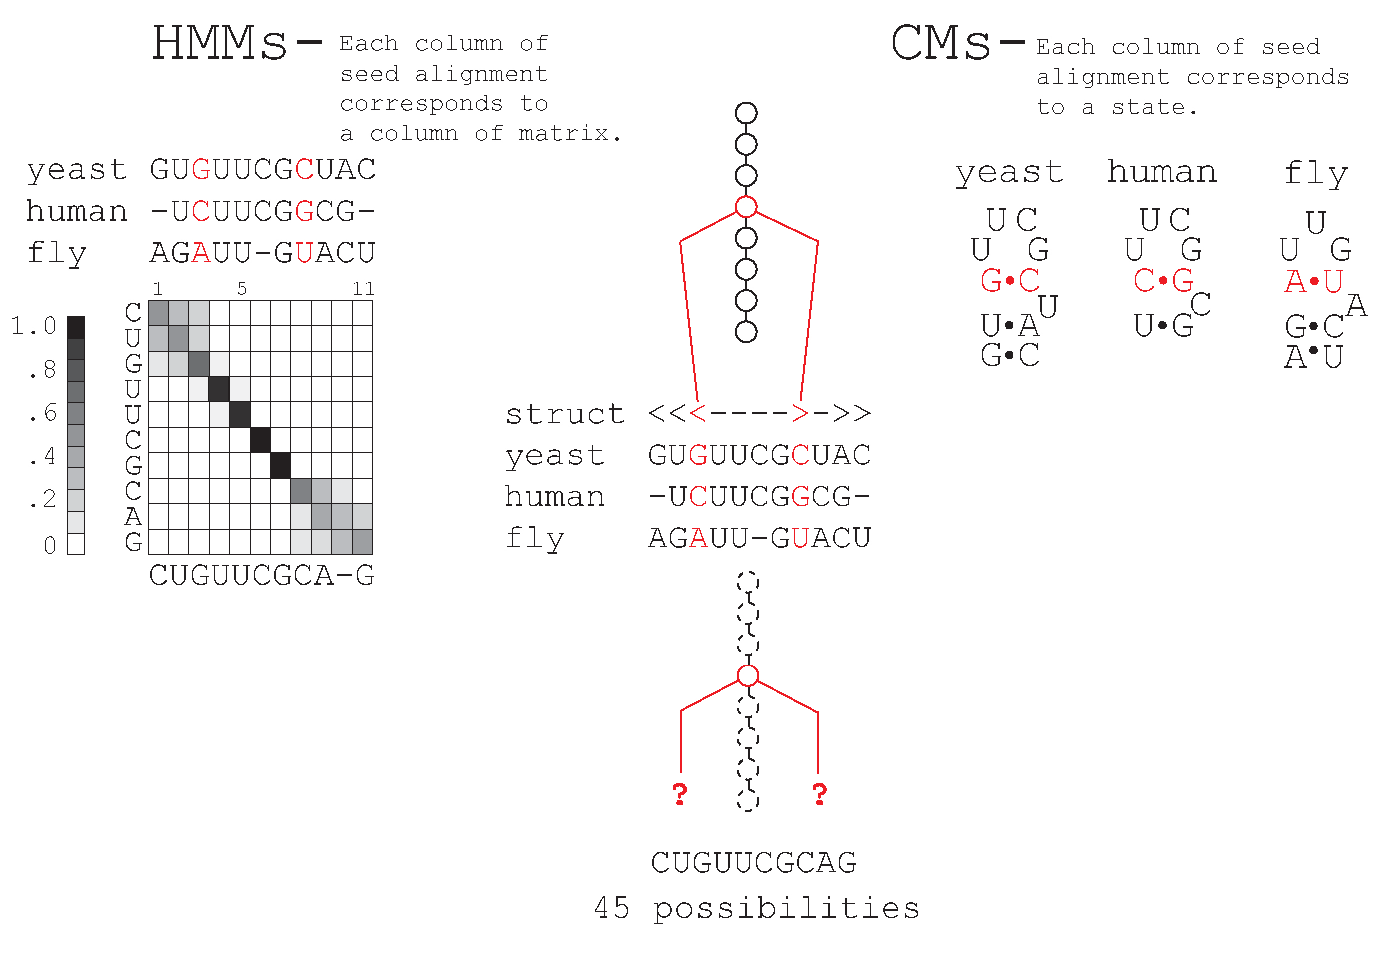
\includegraphics[width=8in]{figs/post_hmm_to_cm_map2_layer14}
\end{center}
\vfill
%\end{minipage}
%\begin{minipage}{4in}
%\vspace{.5in}
%\end{minipage}
\end{slide}
%%%%%%%%%%%%%%%%%%%%%%%%%%%%%%%%%%%%%%%%%%%%%%%%%%%%%%%%%%%%%%%%%%%%%%%%%%
%%%%%%%%%%%%%%%%%%%%%%%%%%%%%%%%%%%%%%%%%%%%%%%%%%%%%%%%%%%%%%%%%%%%%%%%%%
\begin{slide}
\begin{center}

\textbf{HMM bands accelerate CM alignment}
%\textbf{How can we use this information during CM alignment?}
%\textbf{Accelerating CM alignment using HMMs}
\end{center}
\medskip
%\begin{minipage}{6in}
%\begin{center}
%\normalsize
%\textbf{How can we use this information during CM alignment?}
%\end{center}
\small
\begin{itemize}
\item
\textbf{main idea:} eliminate potential alignments the HMM tells us are very improbable
%\item
%restrict which cells of the CM dynamic programming matrix are filled in
%\item
%requires some type of \textbf{map} from the HMM to the CM
%\item
%each single stranded column or base pair from the seed alignment
%corresponds to \\ a face of the 3D CM dynamic programming matrix
\end{itemize}
\begin{center}
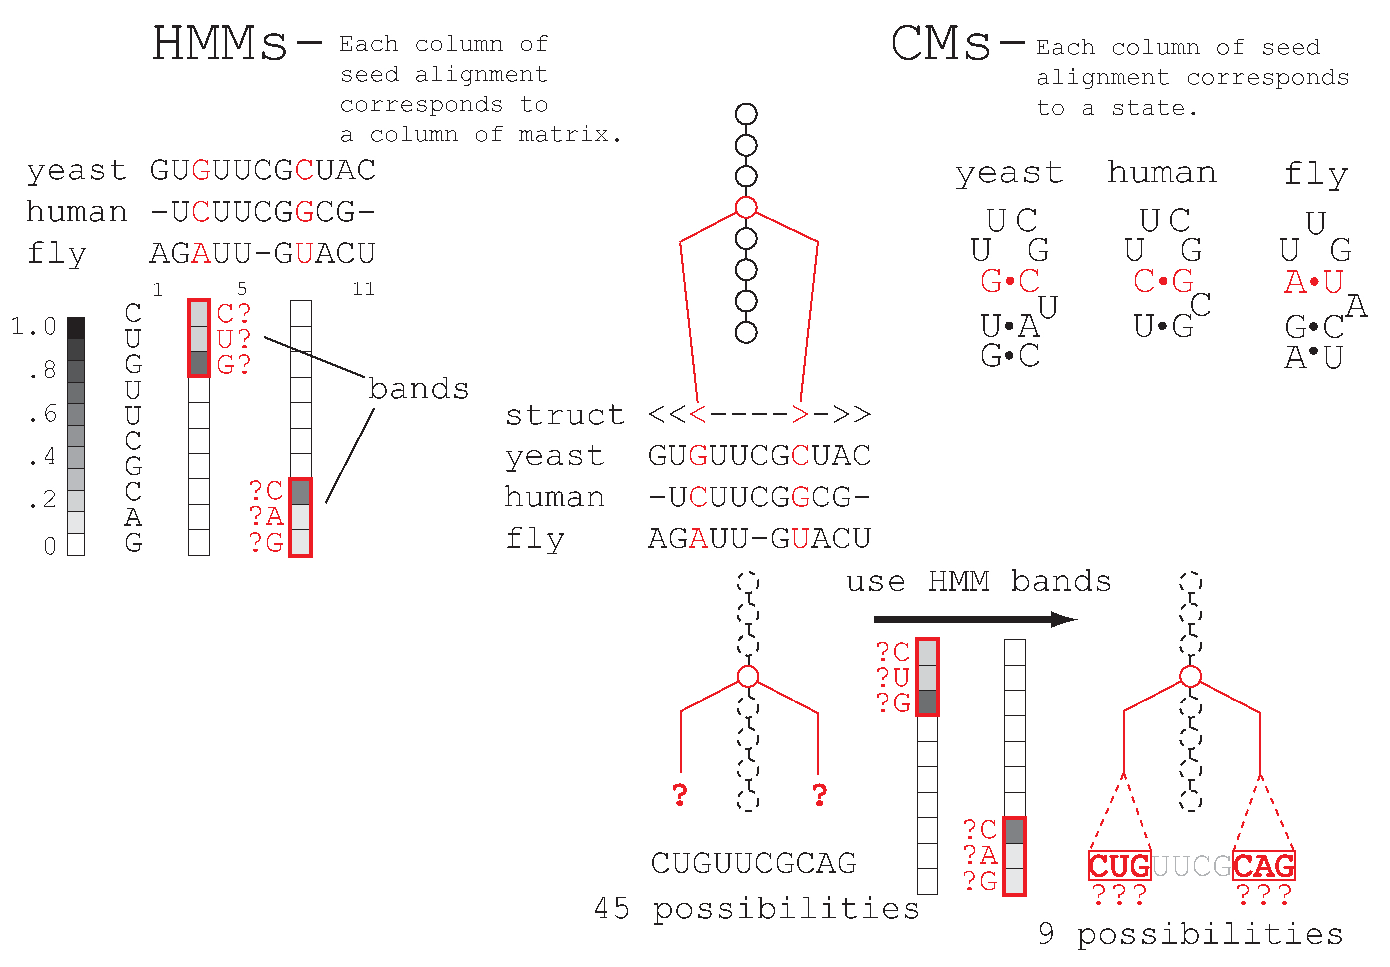
\includegraphics[width=8in]{figs/post_hmm_to_cm_map2_layer16}
\end{center}
\vfill
%\end{minipage}
%\begin{minipage}{4in}
%\vspace{.5in}
%\end{minipage}
\end{slide}
%%%%%%%%%%%%%%%%%%%%%%%%%%%%%%%%%%%%%%%%%%%%%%%%%%%%%%%%%%%%%%%%%%%%%%%%%%


\begin{slide}
\center{\includegraphics[width=10.2in]{figs/roc-2}}
\vfill 
\end{slide}
%%%%%%%%%%%%%%%%%%%%%%%%%%%%%%%%%%%%%%%%%%%%%%%%%%%%%%%%%%%%%%%%%%%%%%%%%%
\begin{slide}

%\center{\includegraphics[width=7in]{figs/menzel09-abstract}}
\center{\includegraphics[width=7in]{figs/menzel09-title}}

\small
\begin{itemize}
\item Searched for 8 RNA families in 26 animal genomes plus
  a choanoflagellate with RNAMotif, ERPIN, BLASTN, and RaveNnA (for non-vertebrates).
\begin{itemize}
\item 
  families: U5, SRP, U3, RNase MRP, let-7, E2, Y, Vault.
\end{itemize}
\item BLASTN does as well or better than other methods in most cases.
\item RaveNnA finds some novel candidates missed by BLASTN in some
  cases, but is very slow.
\end{itemize}

\vfill 
\end{slide}
%%%%%%%%%%%%%%%%%%%%%%%%%%%%%%%%%%%%%%%%%%%%%%%%%
\begin{slide}

\center{\includegraphics[height=6.5in]{figs/fig1-orig-expanded}}

\flushright{\tiny{Menzel et al., Bioinformatics, 2009.}}

\end{slide}
%%%%%%%%%%%%%%%%%%%%%%%%%%%%%%%%%%%%%%%%%%%%%%%%%%%%%%%%%%%%%%%%%%%%%%%%%%
\begin{slide}

\center{\includegraphics[width=10in]{figs/fig1-0729}}

\flushright{\tiny{Modified from Menzel et al., Bioinformatics, 2009.}}

\end{slide}
%%%%%%%%%%%%%%%%%%%%%%%%%%%%%%%%%%%%%%%%%%%%%%%%%%%%%%%%%%%%%%%%%%%%
%%%%%%%%%%%%%%%%%%%%%%%%%%%%%%%%%%%%%%%%%%%%%%%%%%%%%%%%%%%%%%%%%%%%%%%%%%
\begin{slide}

\center{\includegraphics[width=10in]{figs/fig1-plus}}

\flushright{\tiny{Modified from Menzel et al., Bioinformatics, 2009.}}

\end{slide}
%%%%%%%%%%%%%%%%%%%%%%%%%%%%%%%%%%%%%%%%%%%%%%%%%%%%%%%%%%%%%%%%%%%%
%%%%%%%%%%%%%%%%%%%%%%%%%%%%%%%%%%%%%%%%%%%%%%%%%%%%%%%%%%%%%%%%%%%%%%%%%%
\begin{slide}
\begin{center}
\textbf{Running times on all genomes (47 Gb) in hours}
\end{center}
\medskip

\normalsize
\begin{center}
\begin{tabular}{lrrrrrrrr}
  family  &  &    BLASTN  &  &  RNAMotif  &  &     ERPIN  &  &  Infernal \\ \hline
      U5  &  &      0.12  &  &      0.44  &  &      3.68  &  &      8.50 \\
     SRP  &  &      1.82  &  &    120.73  &  &      2.14  &  &    290.94 \\
      U3  &  &      0.09  &  &     35.78  &  &      4.75  &  &     14.18 \\
     MRP  &  &      0.07  &  &      9.16  &  &      6.41  &  &      4.10 \\
   let-7  &  &      0.10  &  &      0.47  &  &     26.80  &  &      3.79 \\
      E2  &  &      0.08  &  &      0.58  &  &      3.16  &  &      4.81 \\
       Y  &  &      0.14  &  &      0.86  &  &    199.16  &  &     11.49 \\
   vault  &  &      0.08  &  &    140.81  &  &     87.67  &  &      4.32 \\\hline
   total  &  &      2.52  &  &    308.83  &  &    333.77  &  &    342.12 \\
\end{tabular}
\end{center}

\vfill
\end{slide}
%%%%%%%%%%%%%%%%%%%%%%%%%%%%%%%%%%%%%%%%%%%%%%%%%%%%%%%%%%%%%%%%%%%%
\begin{slide}
\begin{center}
\textbf{Infernal 1.1} \\ \texttt{infernal.janelia.org}
\end{center}
\medskip

\small
\begin{itemize}
\item faster homology searches
\item no more BLAST filters for Rfam
\item better handling of truncated sequences\footnote{Kolbe and Eddy,
  Bioinformatics, 2009}
\item \texttt{cmscan} program: search a sequence against a CM database
  (e.g. Rfam)
\end{itemize}

\vfill
\end{slide}
%%%%%%%%%%%%%%%%%%%%%%%%%%%%%%%%%%%%%%%%%%%%%%%%%%%%%%%%%%%%%%%%%%%%%%%%%%
%%%%%%%%%%%%%%%%%%%%%%%%%%%%%%%%%%%%%%%%%%%%%%%%%%%%%%%%%%%%%%%%%%
\begin{slide}
\center{\includegraphics[width=10in]{figs/benasque-acknowledgements}}
\vfill
\end{slide}
%%%%%%%%%%%%%%%%%%%%%%%%%%%%%%%%%%%%%%%%%%%%%%%%%%%%%%%%%%%%%%%%%%
\begin{slide}
  \center{\includegraphics[width=10.2in]{figs/roc-1E03}}
\vfill 
\end{slide}
%%%%%%%%%%%%%%%%%%%%%%%%%%%%%%%%%%%%%%%%%%%%%%%%%%%%%%%%%%%%%%%%%%%%%%%%%%
\end{document}
